% Generated figure snippets. Captions state the evidence ceiling explicitly.
\begin{figure*}[t]
  \centering
  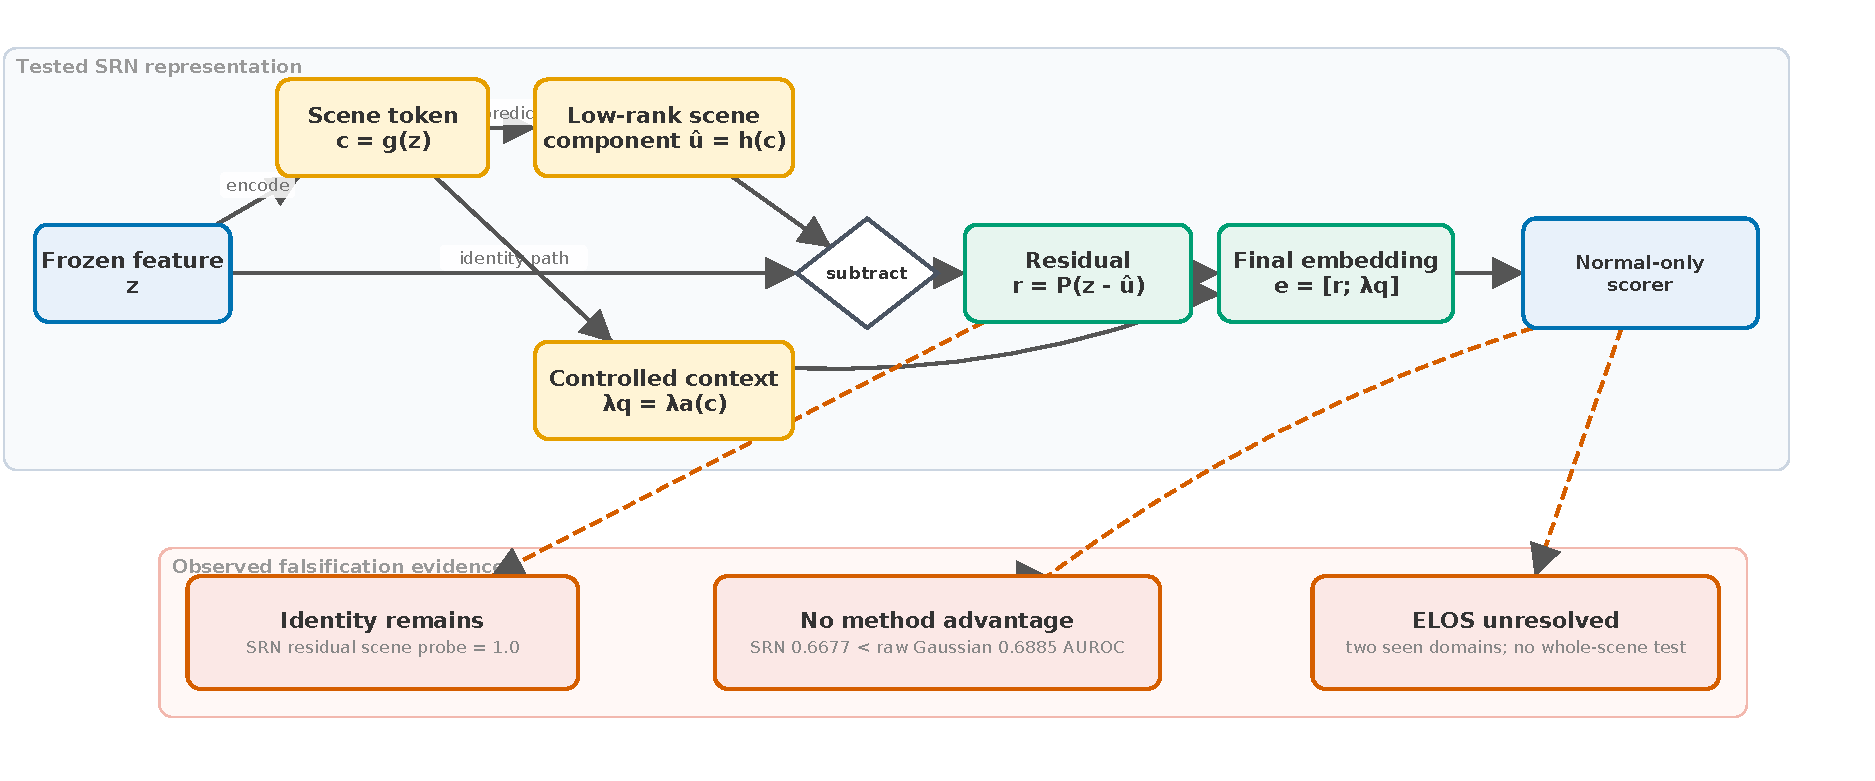
\includegraphics[width=0.98\textwidth]{../figures/fig1_srn_falsification.pdf}
  \caption{The tested SRN hypothesis and its observed falsification. A low-rank scene
  component is predicted, subtracted, and optionally accompanied by controlled context
  before normal-only scoring. On the available two-seen-domain diagnostic, the residual
  retains perfectly decodable domain identity, full SRN trails raw Gaussian scoring, and
  the data cannot establish unseen-scene ELOS.}
  \label{fig:srn_falsification}
\end{figure*}

\begin{figure*}[t]
  \centering
  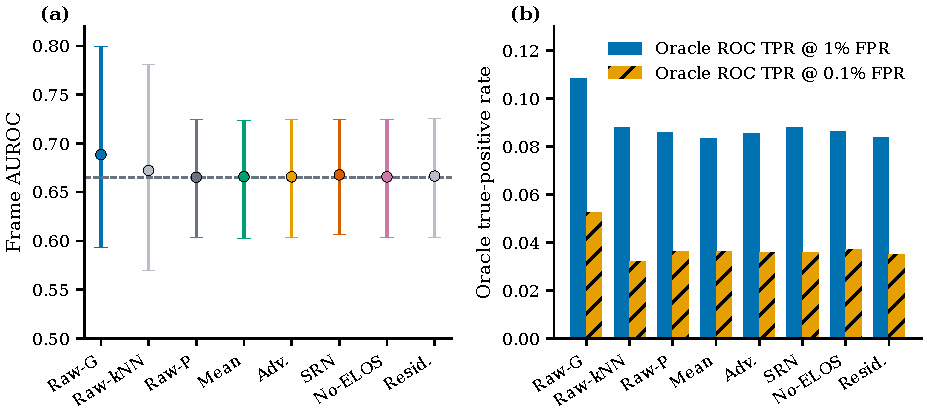
\includegraphics[width=0.95\textwidth]{../figures/fig2_method_comparison.pdf}
  \caption{Joint Ped2+Avenue seen-domain diagnostic. Raw-G, Raw-kNN, and Raw-P denote raw
  Gaussian, kNN, and prototype scorers; Mean is scene-mean subtraction; Adv. is an
  adversarial residual; No-ELOS removes episodic selection; Resid. removes context. (a)
  Frame AUROC with hierarchical video/seed bootstrap intervals; the dashed line is Raw-P.
  (b) Oracle ROC TPRs read using final test labels, not deployable thresholds. Full SRN does
  not outperform Raw-G and overlaps the matched Raw-P baseline.}
  \label{fig:method_comparison}
\end{figure*}

\begin{figure*}[t]
  \centering
  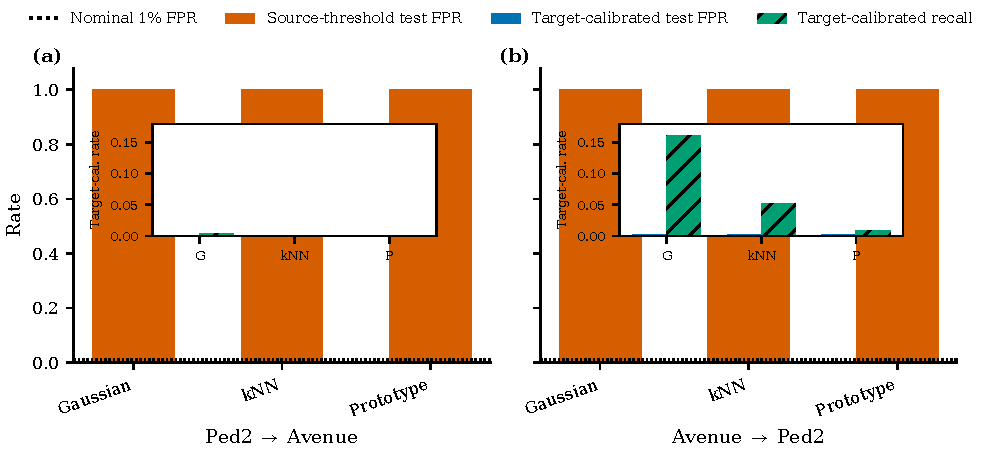
\includegraphics[width=0.90\textwidth]{../figures/fig3_threshold_transfer.pdf}
  \caption{Cross-dataset fixed-threshold reliability. Strict thresholds are selected only
  on source-normal validation; calibrated thresholds use separately declared target-normal
  videos. Every source threshold yields 100\% false positives on target normal frames.
  Target-normal calibration controls false positives but yields low final target-anomaly
  recall, exposing score-distribution shift hidden by rank metrics. Insets magnify the
  calibrated rates (G: Gaussian, P: prototype).}
  \label{fig:threshold_transfer}
\end{figure*}
